\documentclass[letter]{article}
\usepackage[utf8]{inputenc}

% \usepackage{tikz}
\usepackage{graphicx}
\usepackage{wrapfig}
% \usepackage{booktabs}

\usepackage{microtype}

\usepackage{mhsetup}
\usepackage{mathtools}

\usepackage{amssymb}
\usepackage{textcomp}
\usepackage{siunitx}

\usepackage[parfill]{parskip}
\usepackage{array}
% \usepackage{multirow}

\sisetup{
  separate-uncertainty,
  multi-part-units = brackets,
  bracket-numbers,
  sticky-per
}
\numberwithin{equation}{section}
\numberwithin{figure}{section}
\numberwithin{table}{section}
\graphicspath{ {./images/} }


\title{Experiment 7 — Standing waves in water}
\author{Laurence Amadeus Tristan, Nero Su, Weihong Deng}
\date{28/02/2019}

\begin{document}
\maketitle

\section{Purpose}
The purpose of this experiment is to figure out the speed of sound by examining the resonances of an open-ended resonance tube.

\section{Theory}
A standing wave consists two traveling waves interfering with each other in a particular manner that makes it appear stationary as a whole. As such, they consist of both nodes and antinodes. Nodes are positions where the particles in the air are stationary and not moving, whereas antinodes are the opposite of nodes, where the air particles moves back and forth at its greatest amplitude possible. One such example of a standing wave is resonance.

When resonance (i.e. standing waves) occurs, there will be a series of antinodes and nodes set in fixed locations along the air column.  This happens when the length of the air column \(L\) and the wavelength of the sound \(\lambda\) satisfies the equation:

\begin{equation} \label{eq:t1}
  L = N \ \frac{\lambda}{4}, \qquad N = \{1, 3, 5, \ldots\}
\end{equation}

\begin{tabbing}
  where \= \(L\) \= = length of air column, \\
  \> \(N\) \> = resonance order (odd integer values only, e.g. 1, 3, 5, \ldots), \\
  \> \(\lambda\) \> = wavelength of sound.
\end{tabbing}

Note that the length of the air column \(L\) does not equal to the length of the air chamber \(D\) in the tube, as the final antinode is located a distance \(x\) away from the open end of the tube. In terms of \(D\), this means that

\begin{equation} \label{eq:t2}
  L = D + x
\end{equation}

\begin{tabbing} \nopagebreak[3]
  where \= \(L\) \= = length of air column \\
  \> \(D\) \> = length of the air chamber, \\
  \> \(x\) \> = end correction.
\end{tabbing}

The end correction \(x\) is constant. This value depends on the diameter of the tube and the particular sound frequency that is made by the source, and cannot be dependent on the resonance order \(N\).

\section{Procedure}
\begin{wrapfigure}{r}{0.4\textwidth}
  \centering
  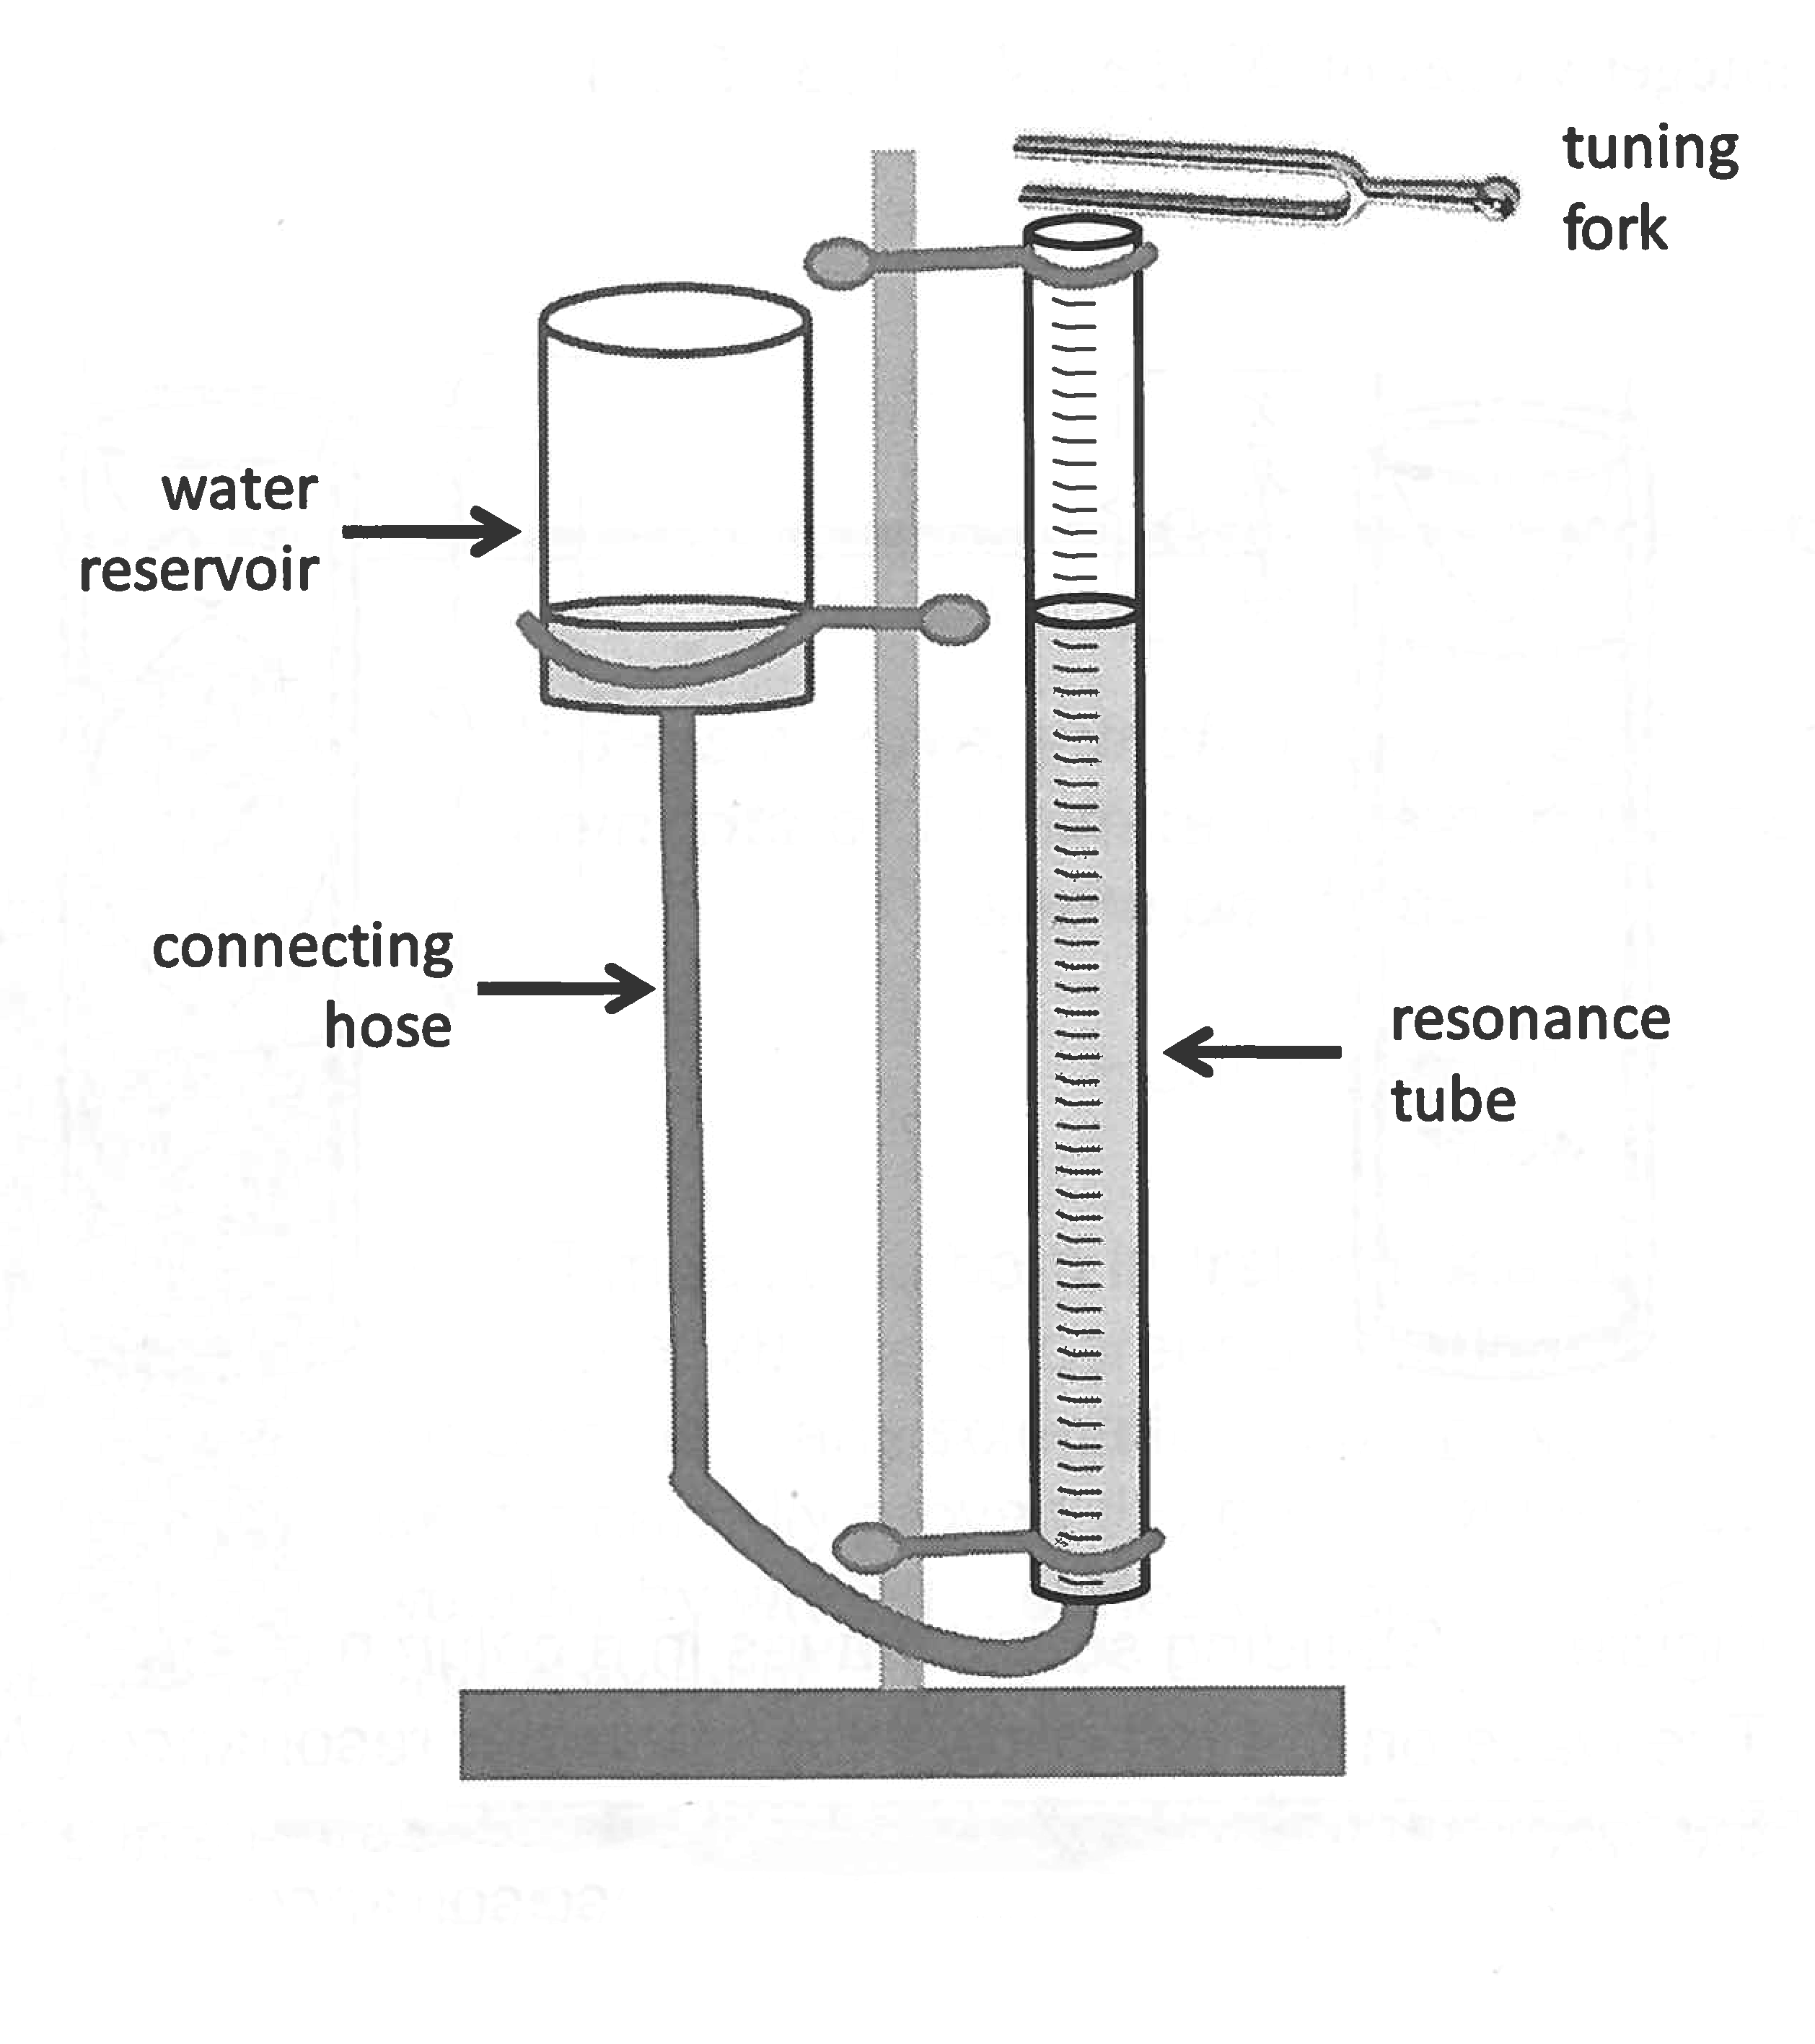
\includegraphics[width=0.4\textwidth]{drawing.png}
  \caption{Diagram of the apparatus}
  \label{fig:apparatus}
\end{wrapfigure}

Before starting the experiment, we first moved the apparatus to the floor of the laboratory. This was done to minimise the chance of breaking the apparatus due to human error. After that, we added a relatively small amount of water to the resevoir in order to increase the range of measurement.

First, we lower the water level in the tube as fast as possible by lowering the resevoir by hand (as in removed from the stand it was placed in). While doing so, gently strike a tuning fork with a rubber mallet and place it just above the resonance tube, taking great care to make sure that the fork do not make contact with the tube. This allows us to locate roughly the values of \(D\) of which resonance happens (in which it will give out a greatly amplified tone of the tuning fork).

Then, using our initial estimates for \(D\), we adjusted the water level so that it matches up with one of our estimates, and with a gently-struck tuning fork, we adjusted the water level continually until we found the value of \(D\) for which the tone experienced the most amplification. Repeat for the other estimates.

After that, we repeated the above procedures for every tuning fork that was provided. Those are listed at \ref{table:d1}. Note that for every \(D\) values that has resonance occuring, those value corresponds to the resonance order \(N\), which has been defined in Equation \eqref{eq:t1}. For most of the tuning forks available to us, only \(N = 1\) and \(N = 3\) resonances were observed, and \(N = 5\) was only observed for the tuning fork with the highest frequency.

\pagebreak
\section{Data}
\begin{table}[!h]
  \setlength\extrarowheight{2.5pt}
  \centering
  \begin{tabular}{|c|c|c|}
    \hline
    Experiment      & Note value            & Frequency (\(f\))/\(\pm 0.1\) \si{Hz} \\
    \hline
    1               & \(\mathrm{F}_4\)      & 349.2 \\
    2               & \(\sim \mathrm{G}_4\) & 392.0 \\
    3               & \(\sim \mathrm{A}_4\) & 486.7 \\
    4               & \(\mathrm{C}_5\)      & 523.2 \\
    \hline
  \end{tabular}
  \caption{Description of each experiment}
  \label{table:d1}
\end{table}

\begin{table}[!h]
  \setlength\extrarowheight{2.5pt}
  \centering
  \begin{tabular}{|c|c|l|}
    \hline
    Variable  & Value                       & Description\\
    \hline
    \(T_C\)   & \SI{24(1)}{\celsius}        & {Room temperature in Celsius}\\
    \(d\)     & \SI{3.366(2)}{\centi\metre} & {Inner diameter of the resonance tube}\\
    \(v_0\)   & \SI{331}{\metre\per\second} & {Speed of sound in air at \SI{0}{\celsius} (\SI{273}{\kelvin})}\\
    \hline
  \end{tabular}
  \caption{List of measured constant variables in the experiment}
  \label{table:d2}
\end{table}

\begin{table}[!h]
  \setlength\extrarowheight{2.5pt}
  \centering
  \begin{tabular}{|c|c|c|c|c|}
    \hline
    \(N\) & \(D_1 / \pm 1\) \si{cm} & \(D_2 / \pm 1\) \si{cm} & \(D_3 / \pm 1\) \si{cm} & \(D_4 / \pm 1\) \si{cm} \\
    \hline
    1  & 24  & 21  & 19  & 15 \\
    3  & 73  & 65  & 59  & 48 \\
    5  & --  & --  & --  & 81 \\
    \hline
  \end{tabular}
  \caption{Experimental data for all four experiments}
  \label{table:d3}
\end{table}

\section{Analysis}
Combine \eqref{eq:t1} and \eqref{eq:t2} and solve for \(D\).

\begin{align} \label{eq:a1}
  \frac{N \lambda}{4} &= D + x \notag \\
  -D &= - \left (\frac{N \lambda}{4} \right) + x \notag \\
  D &= N \left(\frac{\lambda}{4} \right) - x
\end{align}

\pagebreak[3]

As the wavelength \(\lambda\) is constant for each tuning fork, we can safely assume that Equation \ref{eq:a1} is linear. As such, \(\frac{\lambda}{4}\) is the gradient of the linear function, and the error correction \(x\) is the \textit{y}-intercept of the function. As such, for brevity we do the following substitution: \nopagebreak[4]

\begin{equation} \label{eq:a2}
  m = \frac{\lambda}{4}
\end{equation}

With the data from Table \ref{table:d3} (and after converting the measurements to metres) and Equation \ref{eq:a1}, we were able to draw Figure \ref{fig:plot1} of \(D_4\) as a function of \(N\).

\begin{figure}[!h]
  \centering
  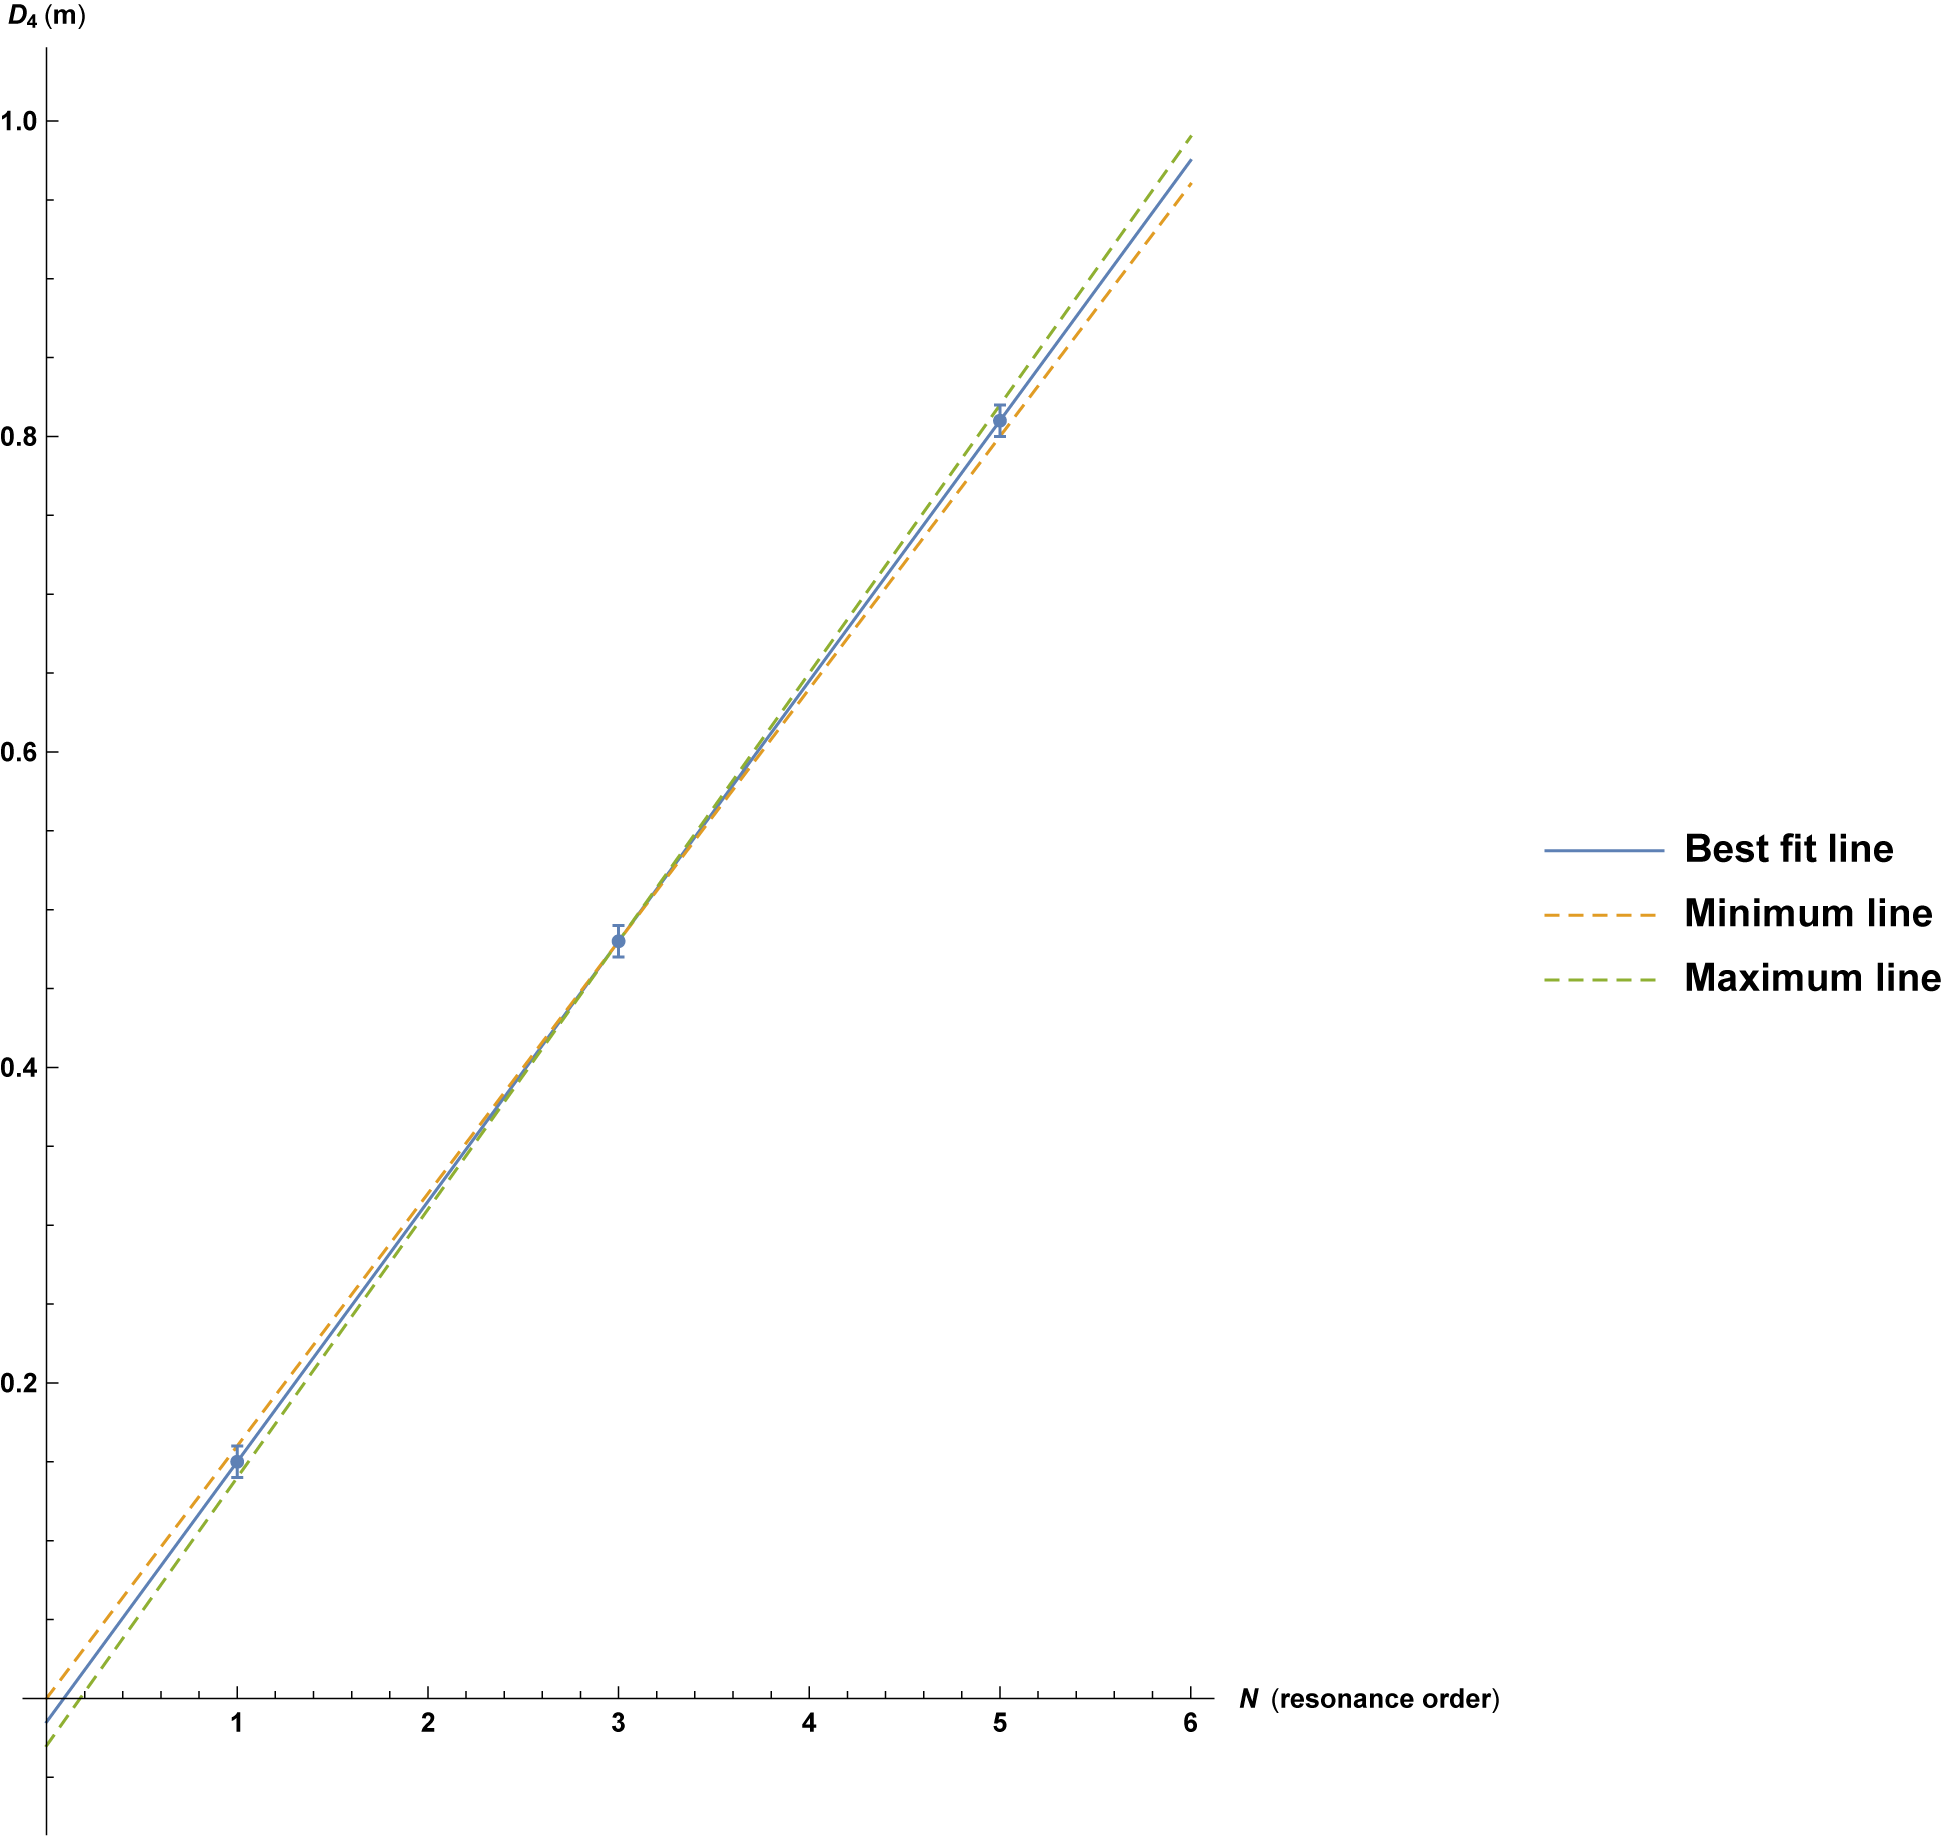
\includegraphics[width=0.75\textwidth]{plot_pdf.png}
  \caption{Plot of the length of air column \(D_4\) against the resonance order \(N\).}
  \label{fig:plot1}
\end{figure}

Now, find out the gradient \(m\) for Experiment 4.

\begin{align*}
  \begin{split}
    m_4 &= \frac{\SI{0.81}{m} - \SI{0.15}{m}}{5 - 1} \\
    &= \SI{0.165}{m}
  \end{split}
  \begin{split}
    \delta m &= m_{\mathrm{best}} - m_{\mathrm{min}} \\
    &= \frac{\SI{0.81}{m} - \SI{0.15}{m}}{5 - 1} - \frac{\SI{0.80}{m} - \SI{0.14}{m}}{5 - 1} \\
    &= \SI{0.165}{m} - \SI{0.16}{m} \\
    &= \SI{0.005}{m}
  \end{split}
\end{align*}

\[\therefore m_4 = \SI{0.165(5)}{m}\]

\pagebreak

With \eqref{eq:a2}, find \(\lambda\) using the value of \(m\) for Experiment 4.
\begin{align} \label{eq:a3}
  m &= \frac{\lambda}{4} \notag \\
  \lambda &= 4m
\end{align}

\nopagebreak

\begin{align*}
  \begin{split}
    \lambda_4 &= 4m_4 \quad \text{[with \eqref{eq:a3}]} \\
    \lambda_4 &= 4(\SI{0.165}{m}) \\
    &= \SI{0.66}{m}
  \end{split}
  \begin{split}
    \delta \lambda &= |4| \delta m \\
    &= |4| (\SI{0.005}{m}) \\
    &= \SI{0.02}{m}
  \end{split}
\end{align*}
\[\therefore \lambda_4 = \SI{0.66(2)}{m}\]

From Figure \ref{fig:plot1}, get the value of \(x\) along with its uncertainty.
\begin{align*}
  x &= \SI{0.015}{m}, \\
  x_\mathrm{min} &= \SI{0}{m}
\end{align*}
\begin{align*}
  \delta x &= |x_{\mathrm{best}} - x_{\mathrm{min}}| \\
  &= |\SI{0.015}{m} - \SI{0}{m}| \\
  &\approx \SI{0.02}{m}
\end{align*}
\[\therefore x = \SI{0.02(2)}{m}\]

For the rest of the experimental data (Experiment 1 to 3), we assume that the best-fit line goes through the two data points. The uncertainties for the values of \(\lambda\) and \(x\) can be assumed to be similar, if not identical, for all forks. Because of that, the calculations needed to determine \(m\), \(\lambda\), and \(x\) are quite similar to the calculations done for Experiment 4. The following is an example calculation for Experiment 1:

\begin{align*}
  \begin{split}
    m_1 &= \frac{\SI{0.73}{m} - \SI{0.21}{m}}{3 - 1} \\
    &= \SI{0.26}{m}
  \end{split}
  \begin{split}
    \lambda_1 &= 4(\SI{0.26}{m}) \\
    &= \SI{1.04(2)}{m}
  \end{split} \\
\end{align*}
\begin{equation*}
  \begin{split}
    D_1 &= m_1 N - x_1 \\
    x_1 &= -D_1 + m_1 N \\
    &= \SI{-0.73}{m} + (\SI{0.26}{m})(3) \\
    &= \SI{0.05(2)}{m}
  \end{split}
\end{equation*}

Note that in the case for Experiments 1--3, the values above for \(m, \ \lambda, \) and \(x\) are determined algrbraically (unlike Experiment 4).

\begin{table}[h]
  \setlength\extrarowheight{2.5pt}
  \centering
  \begin{tabular}{|c|c|c|c|c|}
    \hline
    Experiment & {\(f\)/\si{\hertz} }& {\(\lambda\)/\si{m}} & {\(x\)/\si{m}} & {\(v\)/\si{m.s^{-1}}} \\
    \hline
    1 & \num{349.2(1)} & \num{1.04(2)} & \num{0.05(2)} & \num{363(7)} \\
    2 & \num{392.0(1)} & \num{0.88(2)} & \num{0.01(2)} & \num{345(8)} \\
    3 & \num{486.7(1)} & \num{0.80(2)} & \num{0.01(2)} & \num{390(10)} \\
    4 & \num{523.2(1)} & \num{0.66(2)} & \num{0.02(2)} & \num{350(10)} \\
    \hline
  \end{tabular}
  \caption{Processed experimental data}
  \label{table:a1}
\end{table}

The speed of sound \(v\) for each experiment is found using
\begin{align} \label{eq:a4}
  \begin{split}
    v = f \lambda
  \end{split}
  \begin{split}
    \delta v = v \left(\frac{\SI{0.1}{Hz}}{f} + \frac{\SI{0.02}{m}}{\lambda} \right)
  \end{split}
\end{align}
and inputting the values of \(f\) and \(\lambda\) for each experiment, accounting for the uncertainties for both \(f\) and \(\lambda\). From the \(v\) values in Table \ref{table:a1}, we can find the mean of \(v\) along with its uncertainty.

\begin{align*}
  \begin{split}
    \bar{v} &= \frac{\SI{363}{\metre\per\second} + \SI{345}{\metre\per\second} + \SI{390}{\metre\per\second} + \SI{350}{\metre\per\second}}{4} \\
    &= \SI{362}{\metre\per\second}
  \end{split} \\
  \begin{split}
    \delta \bar{v} &= \frac{1}{4} (\delta v_1 + \delta v_2 + \delta v_3 + \delta v_4) \\
    &= \frac{1}{4} (\SI{7}{\metre\per\second} + \SI{8}{\metre\per\second} + \SI{10}{\metre\per\second} + \SI{10}{\metre\per\second}) \\
    &= \SI{8.75}{\metre} \\
    &\approx \SI{9}{\metre}
  \end{split}
\end{align*}
\[\therefore \bar{v} = \SI{362(9)}{\metre\per\second}\]

Now, let's compare \(\bar{v}\) to the theoretical value of the speed of sound \(v_{\mathrm{s}}\) at \SI{24}{\celsius}. From Table \ref{table:d2}, at \SI{0}{\celsius} (\SI{273}{\kelvin}) the speed of sound \(v_0\) is \SI{331}{\metre\per\second}. This value depends on the average velocity of the air particles. As temperature increases the average velocity increases as well, which means the speed of sound increases with temperature too. To fiugre out the speed of sound at the temperature \(T\) (in kelvins), we use the following formula:

\begin{equation} \label{eq:a5}
  v_{\mathrm{s}} = v_0 \sqrt{\frac{T}{\SI{273}{\kelvin}}}
\end{equation}

\begin{tabbing}
  where \= \(v_{\mathrm{s}}\) \= = speed of sound at temperature \(T\), \\
  \> \(v_0\) \> = speed of sound at \SI{273}{\kelvin}, \\
  \> \(T\) \> = temperature of room in kelvins.
\end{tabbing}

After converting the value of \(T_C\) to kelvins, find the theoretical speed of sound at the room temperature.

\begin{align} \label{eq:a6}
  T &= 273 + T_C \\
  &= 273 + 24 \notag \\
  &= \SI{297(1)}{\kelvin} & \text{[uncertainty remains identical]} \notag
\end{align}
From \eqref{eq:a5} and data from both Table \ref{table:d2} and the calculation above,
\begin{align*}
  \begin{split}
    v_{\mathrm{s}} &= \SI{331}{\metre\per\second} \sqrt{\frac{\SI{297}{\kelvin}}{\SI{273}{\kelvin}}} \\
    &= \SI{345.2430104}{\metre\per\second}
  \end{split}
  \begin{split}
    \delta v_{\mathrm{s}} &= v_{\mathrm{s}} \left[\frac{1}{2} \left( \frac{\SI{1}{\kelvin}}{\SI{297}{\kelvin}} \right)  \right] \\
    &= \SI{0.5812171893}{\metre\per\second} \\
    &\approx \SI{0.6}{\metre\per\second}
  \end{split}
\end{align*}
\[\therefore v_{\mathrm{s}} = \SI{345.2(6)}{\metre\per\second}.\]

Find out how far our experimentally-derived speed of sound \(\bar{v}\) is from the theoretical speed of sound \(v_{\mathrm{s}}\).

\begin{align*}
  \mathrm{\%\ Discrepancy} &= \frac{\SI{362}{\metre\per\second} - \SI{345.2}{\metre\per\second}}{\SI{345.2}{\metre\per\second}} \times 100 \\
  &\approx 4.9\%
\end{align*}

For the end correction \(x\), we can compare those experimental values with an approximate, like the following:

\begin{equation} \label{eq:a7}
  x_{\mathrm{approx}} \approx 0.82r
\end{equation}

\begin{tabbing}
  where \= \(x_{\mathrm{approx}}\) \= = end correction, \\
  \> \(r\) \> = radius of tube.
\end{tabbing}

In our case we are going to intepret "radius of tube" to mean the inner radius of the resonance tube, which we have measured in Section 3 as the inner diameter of the tube (Table \ref{table:d2}). However we need to get the inner radius of the tube.

\begin{align*}
  d &= 2r \\
  r &= \frac{d}{2} \\
  &= \frac{\SI{3.366(2)d-2}{\metre}}{2} \\
  &= \SI{1.683(1)d-2}{\metre}
\end{align*}

Using \eqref{eq:a7} and \(r\), get an approximation of \(x\) based on the inner radius of the tube. Note that since this is an approximation we shall drop the uncertainty as it will give a false sense of accuracy.
\nopagebreak[3]
\begin{align*}
  x_{\mathrm{approx}} &\approx 0.82(\SI{1.683d-2}{\metre}) \\
  &= \SI{1.3801d-2}{\metre}
\end{align*}

After that we calculate the difference between the \(x\)-values for each frequency with the approximation that we have obtained.

\begin{table}[!h]
  \setlength\extrarowheight{2.5pt}
  \centering
  \begin{tabular}{|c|c|c|}
    \hline
    Experiment & {\(x\)/\(\pm 0.02\) \si{\metre}} & Difference/\si{m} \\
    \hline
    1 & 0.05 & 0.04 \\
    2 & 0.01 & 0.004 \\
    3 & 0.01 & 0.004 \\
    4 & 0.02 & 0.006 \\
    \hline
  \end{tabular}
  \label{table:a2}
  \caption{Difference of the value of the end correction \(x\) between experimental result and the approximation suggested by \eqref{eq:a7}}
\end{table}

To calculate:

\begin{equation}
  \text{Difference} = |x - x_{\mathrm{approx}}|
\end{equation}

\section{Discussion}
In this experiment, we attempted to measure the speed of sound \(v\) by examining the resonances of an open-ended resonance tube. We did this by first manipulating Equation \ref{eq:t1} and \ref{eq:t2} to produce \eqref{eq:a1} along with \eqref{eq:a2}. Then, we figure out the values of \(m\) and \(x\) and used those values along with Equation \ref{eq:a3} \(\lambda\). With \eqref{eq:a4} \(\lambda\) is then used (along with its corresponding \(f\)) to find the speed of sound for each experiment/frequency, which then used to find \(\bar{v}\). We then compared the mean speed of sound \(\bar{v}\) with a theoretical value of the speed of sound \(v_\mathrm{s}\). Lastly we then compared the end corrections that we got for each frequencies with an approximation that has been suggested.

From the experiment, we found that the mean experimental speed of sound \(\bar{v}\) is \SI{362(9)}{\metre\per\second}, which differs from the theoretical value of the speed of sound \(v_{\mathrm{s}}\) (\SI{345.2(6)}{\metre\per\second}) by about 4.9\%, which is outside the error of \(\pm\ 9\) \si{\metre\per\second}. As such we consider our value for the speed of sound to be inaccurate.

We suspect there are many factors that contributes to the inaccurate value of \(\bar{v}\). One of those is the difficulty of pinpointing the exact \(D\) value for which resonance happens. In our case we were relying on our human hearing to determine at what point along the tube that the tone has been maximally amplified. This is quite problematic as in this case we can only determine ``peak" loudness (i.e. the value of \(D\) when resonance happens) subjectively, with no way of knowing exactly what values of \(D\) has the highest sound level.

Another factor is the lack of repetition for the measurement of \(D\) for all observed resonance orders (\(N = \{1, \ 3, \ 5\}\)), which can help reduce the uncertainty of each data point and may increase accuracy. We also noticed that the tube that was supplied was not long enough to capture the fifth resonance order for experiments 1, 2, and 3. There's also a slight tilt on the resonance tube, however we only noticed it after finishing the experiments.

We have several suggestions to the experiment in order to improve the accuracy Firstly, add at least \SI{30}{\cm} to the length of the tube. This potentially allows us to measure the fifth resonance order of the lower frequencies and therefore allow us to have at least three data points for all four experiments. We would also suggest correcting the tilt on the resonance tube, howerver we suspect that it might have minimal-to-no impact on accuracy. Lastly, we suggest repeating the experiment at least three times in order to decrease the chance of any random errors occuring.

\end{document}